\documentclass[aspectratio=169]{beamer}
\usetheme{metropolis}

\usepackage{esdiff}
\usepackage{siunitx}
\usepackage{minted}
\setminted{fontsize=\scriptsize}

\title{BrainScaleS Workshop}
\subtitle{4th HBP School}

\date{\today}
\author{Korbinian Schreiber \& Sebastian Billaudelle}
\institute{Kirchhoff-Institute for Physics, Heidelberg University}

\newcommand*\circled[1]{\tikz[baseline=(char.base)]{
	\node[shape=circle,fill=white,draw=mDarkTeal,inner sep=3pt] (char) {\color{white}\textbf{#1}};
	\node[shape=circle,fill=mDarkTeal,inner sep=2pt] (char) {\color{white}\textbf{#1}};
	}}

\begin{document}

\maketitle

\section{First Section}

{
\usebackgroundtemplate{
\includegraphics[width=\paperwidth]{assets/three_column_background.pdf}}%
\begin{frame}[fragile]
	\frametitle{Analog Neuromorphic Hardware}

	\vspace{-30pt}
	\begin{columns}
		\column{0.33\paperwidth}
		\begin{center}
			\circled{1}
			\vspace{20pt}

			observations
		\end{center}
	
		\column{0.33\paperwidth}
		\begin{center}
			\circled{2}
			\vspace{20pt}

			mathematical model
		\end{center}
		
		\column{0.33\paperwidth}
		\begin{center}
			\circled{3}
			\vspace{20pt}

			hardware realization
		\end{center}
	\end{columns}

	\vspace{10pt}
	
	\begin{columns}
		\column{0.33\paperwidth}
		\begin{center}
			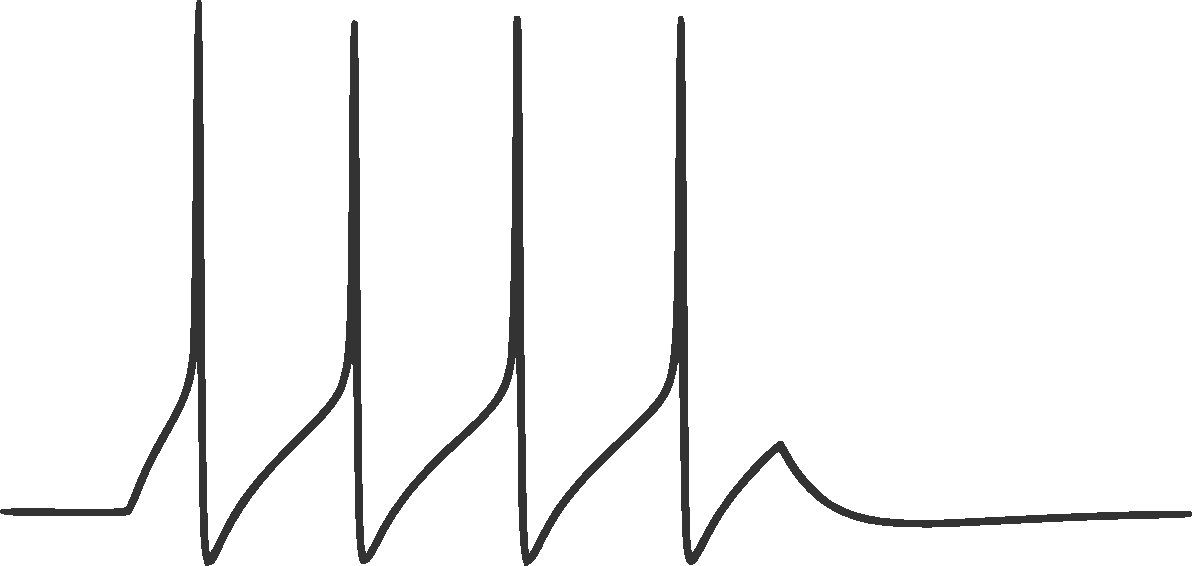
\includegraphics[width=0.8\textwidth]{assets/trace.pdf}
		\end{center}
	
		\column{0.33\paperwidth}
		\begin{center}
			\vspace{-20pt}
			\begin{gather*}
				\scriptstyle
				C \diff{V}{t} = -g_\text{L} \left( V - E_\text{L} \right) + I_\text{syn}(t) \\
			\end{gather*}
		\end{center}
		
		\column{0.33\paperwidth}
		\begin{center}
			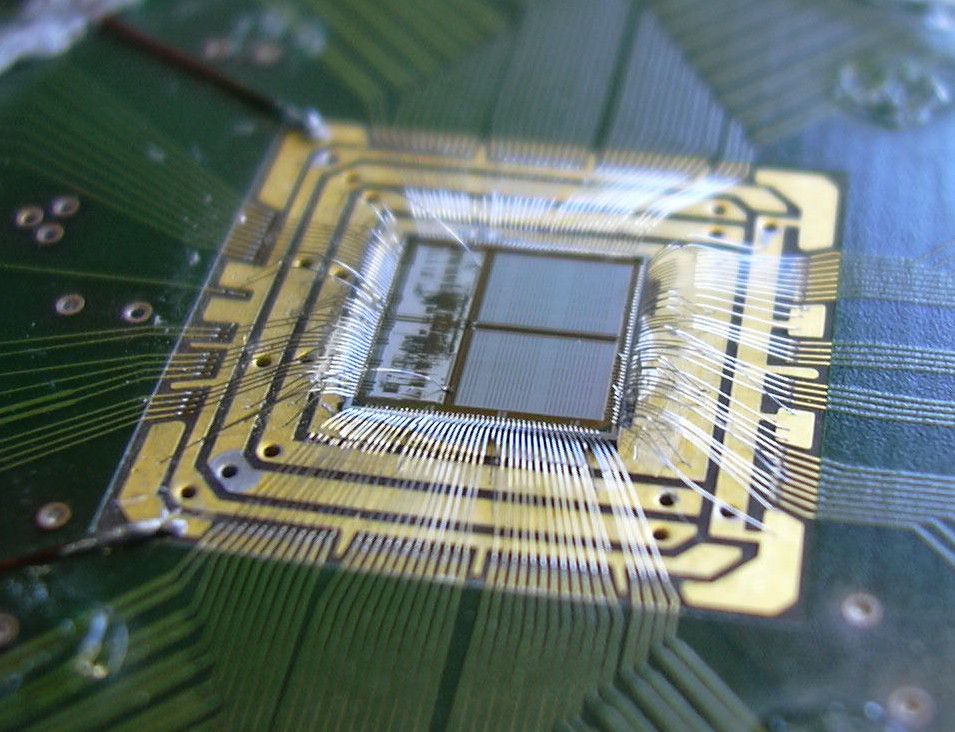
\includegraphics[width=0.8\textwidth]{assets/spikey.jpg}
		\end{center}
	\end{columns}
\end{frame}
}

{
\usebackgroundtemplate{
\includegraphics[width=\paperwidth]{assets/five_column_background.pdf}}%
\begin{frame}[fragile]
	\frametitle{Roadmap}

	\begin{columns}
		\column{0.2\paperwidth}
		\begin{center}
			\circled{2004}
		\end{center}
		\column{0.2\paperwidth}
		\begin{center}
			\circled{2010}
		\end{center}
		\column{0.2\paperwidth}
		\begin{center}
			\circled{2015}
		\end{center}
		\column{0.2\paperwidth}
		\begin{center}
			\circled{2017}
		\end{center}
		\column{0.2\paperwidth}
		\begin{center}
			\circled{2022}
		\end{center}
	\end{columns}

	\vspace{20pt}

	\begin{columns}[T]
		\column{0.2\paperwidth}
		\begin{center}
			\textbf{\color{mDarkTeal}Spikey}
		\end{center}
		\begin{itemize}
				\item single chip system
				\item 384 LIF neurons
		\end{itemize}
		
		\column{0.2\paperwidth}
		\begin{center}
			\textbf{\color{mDarkTeal}HICANN}
		\end{center}
		\begin{itemize}
				\item \SI{180}{\nano\meter} CMOS
				\item 512 AdEx neurons
		\end{itemize}
		
		\column{0.2\paperwidth}
		\begin{center}
			\textbf{\color{mDarkTeal}20 Wafer System}
		\end{center}
		\begin{itemize}
			\item 4 million neurons
			\item 0.9 billion synapses
		\end{itemize}
		
		\column{0.2\paperwidth}
		\begin{center}
			\textbf{\color{mDarkTeal}HICANN DLS}
		\end{center}
		\begin{itemize}
			\item \SI{65}{\nano\meter} CMOS
			\item PPU: integrated processing unit for advanced plasticity
		\end{itemize}
		
		\column{0.2\paperwidth}
		\begin{center}
			\textbf{\color{mDarkTeal}500 Wafer System}
		\end{center}
		\begin{itemize}
			\item 500 million neurons
			\item 130 billion synapses
		\end{itemize}
	\end{columns}
\end{frame}
}

\begin{frame}{PyNN API documentation}
	\begin{center}
		\url{https://neuralensemble.org/docs/PyNN/0.7/api/api-0.7.html}
	\end{center}

	\vspace{3ex}

	Look out for:
	\begin{itemize}
		\item \mintinline{Python}{pynn.Population}
		\item \mintinline{Python}{pynn.Projection}
		\item \mintinline{Python}{pynn.*Connector}
	\end{itemize}
\end{frame}

\begin{frame}[fragile]{Creating (groups of) neurons}
	Create \emph{populations} of neurons:
	\begin{minted}{python}
params = {
    "v_thresh": -60.0
    }
neurons = pynn.Population(42, pynn.IF_facets_hardware1, cellparams=params)
	\end{minted}

	\vspace{3ex}

	Get a list of default neuron parameters:
	\begin{minted}{python}
print pynn.IF_facets_hardware1.default_parameters
	\end{minted}
\end{frame}

\begin{frame}[fragile]{Generating stimuli}
	Create a stimulus from a spike train:
	\begin{minted}{python}
spike_train = np.arange(10.0, 101.0, 10.0)
stimulus = pynn.Population(1, pynn.SpikeSourceArray, {"spike_times": spike_train})
	\end{minted}

	\vspace{3ex}

There is also a Poisson spike source:
	\begin{minted}{python}
poisson_params = {
    "start": 10.0,
    "duration": 100.0,
    "rate": 5.0
    }
stimulus = pynn.Population(1, pynn.SpikeSourcePoisson, poisson_params)
	\end{minted}
\end{frame}

\begin{frame}[fragile]{Synaptic connections}
\end{frame}

\begin{frame}[fragile]{Recording observables}
	Spike times:
	\begin{minted}{python}
neurons.record()
...
spikes = neurons.getSpikes()
	\end{minted}

	\vspace{3ex}
	
	\emph{Analog} membrane traces:
	\begin{minted}{python}
pynn.record_v(neurons[0], "")
	\end{minted}
	\begin{itemize}
		\item only \emph{one} analog-to-digital converter (ADC)
		\item[→] one can record a single neuron at a time
	\end{itemize}
\end{frame}

\end{document}
